\section{Results of Individual Improvements in the CSC Trigger Algorithm}
\label{sec:SLHC_algo_results}

This chapter presents results of the study of effects of individual improvements described in Sec.~\ref{sec:SLHC_algo} on the ALCT, CLCT, and LCT reconstruction efficiencies.

The study is performed with Monte Carlo simulation of double muon events mixed with PU400 events, where the simulation includes GEN, SIM, DIGI, L1 steps.

Three are three baseline configurations of L1 step used in this study:
\begin{itemize}
	\item Baseline 1: SLHC configuration, where the maximum set of improvements is turned off bringing it to 2007 configuration as close as possible. 
	There are only two differences between Baseline 1 and 2007 configurations: separate treatments of ME1a and ME1b, and unganging cathode strips in ME1a;
	\item Baseline 2: Baseline 1 configuration with all improvements on the ALCT and CLCT processors level turned on;
	\item SLHC configuration itself.
\end{itemize}

All algorithm improvements devided into three groups and studied with improvements in the given group turned on one by one on top of each other
\begin{itemize}
	\item ALCT processor level
	\item CLCT processor level
	\item TMB level
\end{itemize}

In the first two groups the L1 step configuration gradually changes from Baseline 1 to Baseline 2 configuration, in the last one --- from Baseline 2 to SLHC configuration.

\newpage

\subsection{ALCT Processor Level Improvements}

\begin{figure}[htb]
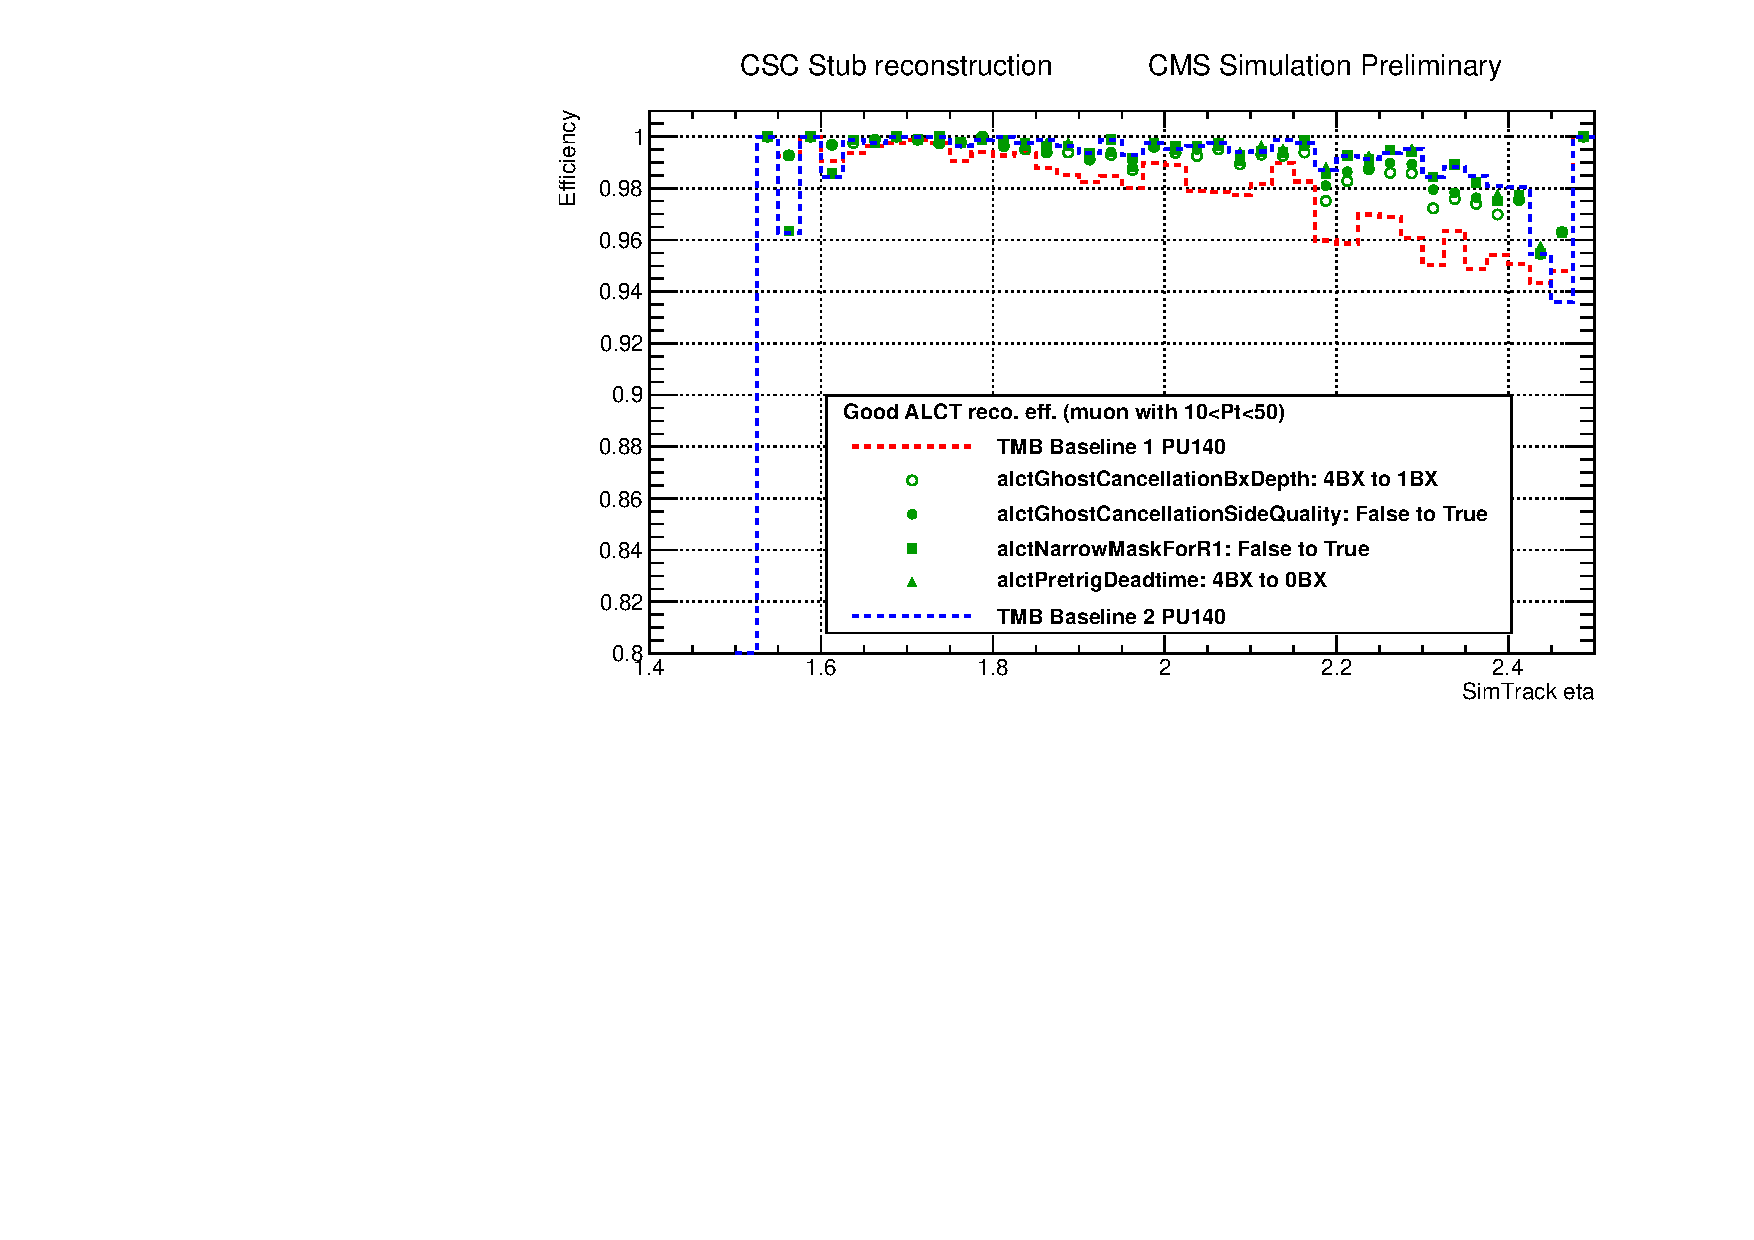
\includegraphics[width=0.98\textwidth]{figures/ALCT_improvements_ALCT_recoEff.pdf}
\caption{Reconstruction efficiency of a good ALCT in ME1 station}
\label{fig:ALCT_improvements_ALCT_recoEff}
\end{figure}

Improvements on the level of ALCT processor are related to the following configuration parameters (see Sec.~\ref{sec:ALCT_conf}):
\begin{itemize}
	\item alctGhostCancellationBxDepth: 4BX to 1BX;
	\item alctGhostCancellationSideQuality: False to True;
	\item alctNarrowMaskForR1: False to True;
	\item alctPretrigDeadtime: 4BX to 0BX.
\end{itemize}

Fig.~\ref{fig:ALCT_improvements_ALCT_recoEff} shows reconstruction efficiency of a good ALCT in ME1 station versus pseudorapidity of the simulated muon for different L1 configurations. The good ALCT is defined as ALCT:
\begin{itemize}
	\item read out in the window of 3BX around the central BX (BX6);
	\item reconstructed within 2 anode wire groups from the key wire group.
	\item has hits at least on three layers
\end{itemize}

The major improvement in ALCT reconstruction efficiency comes from the changes in ALCT ghost cancellation procedure.

\newpage

\subsection{CLCT Processor Level Improvements}

\begin{figure}[htb]
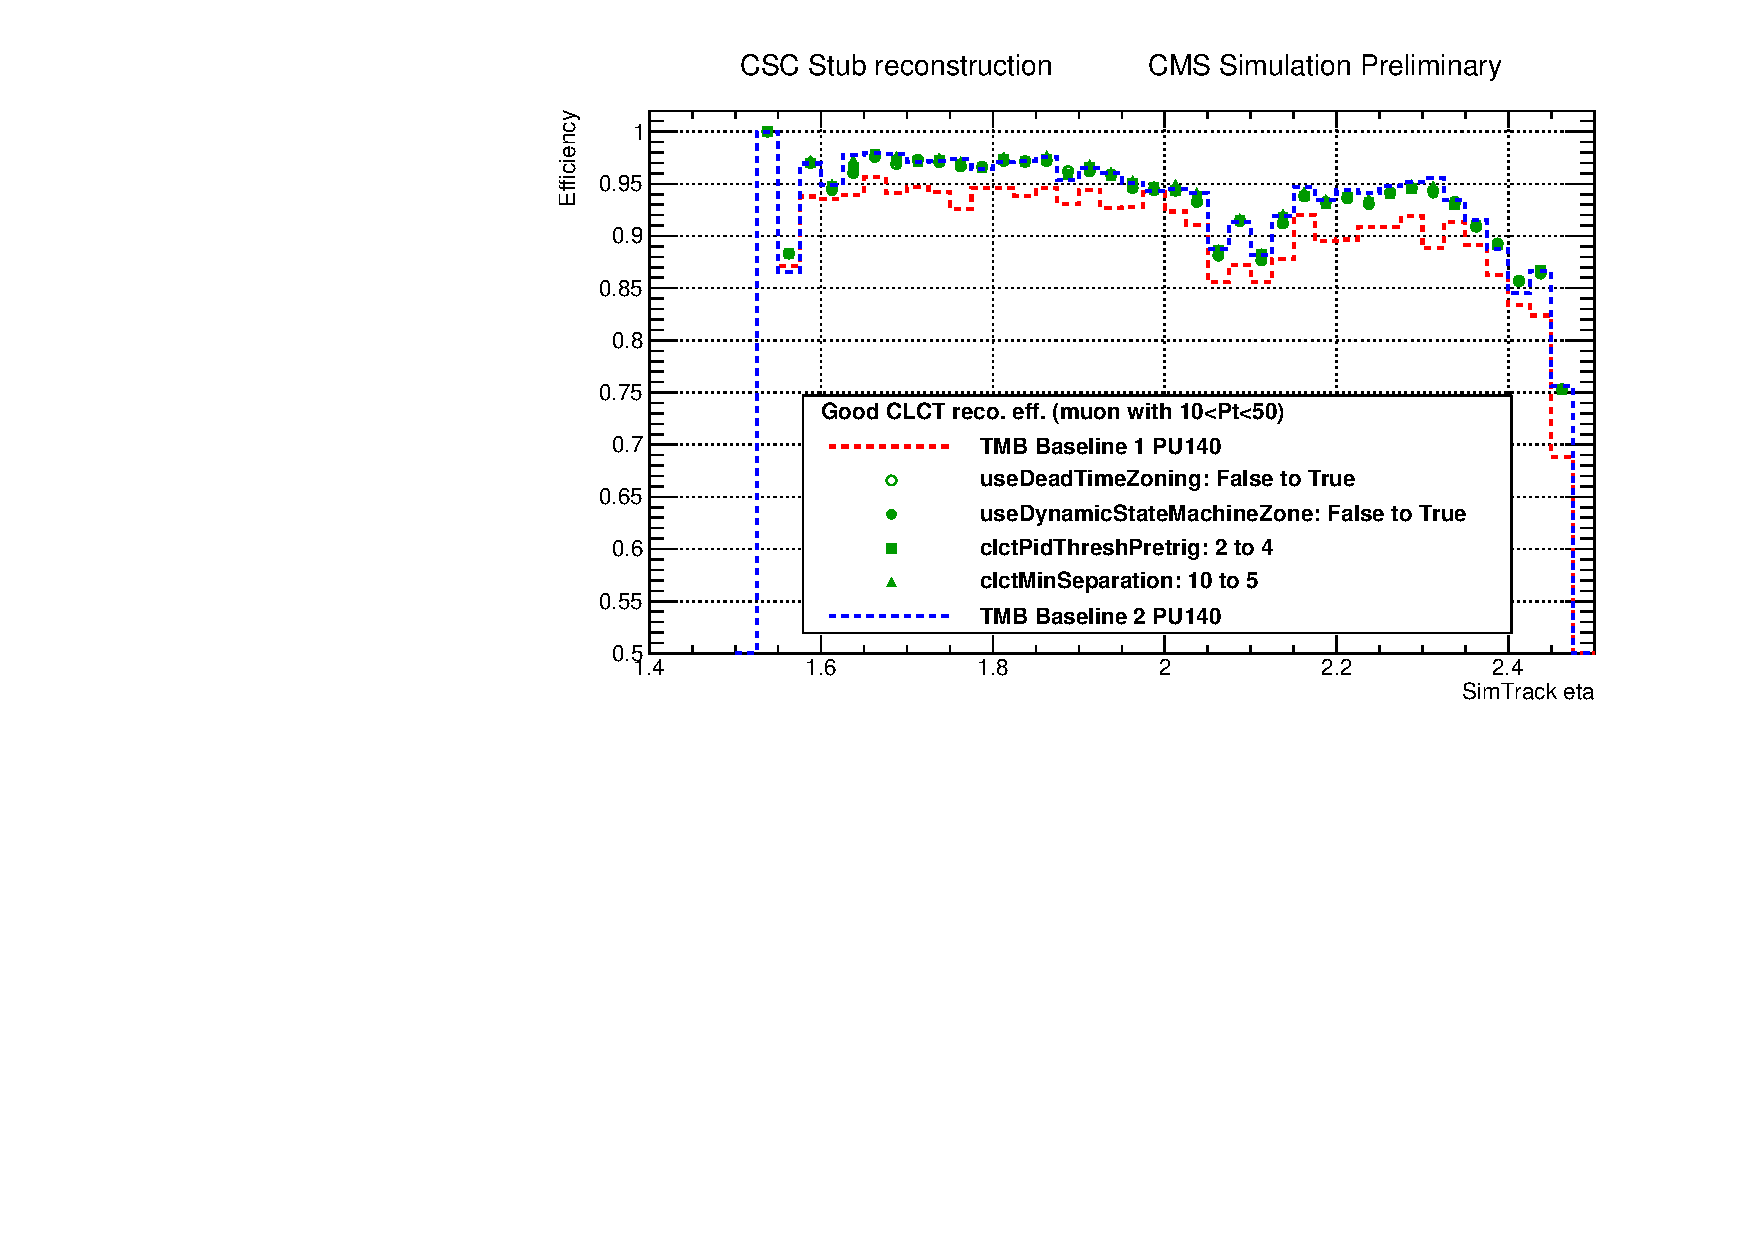
\includegraphics[width=0.98\textwidth]{figures/CLCT_improvements_CLCT_recoEff.pdf}
\caption{Reconstruction efficiency of a good CLCT in ME1 station}
\label{fig:CLCT_improvements_CLCT_recoEff}
\end{figure}

Improvements on the level of CLCT processor are related to the following configuration parameters (see Sec.~\ref{sec:CLCT_conf}):
\begin{itemize}
	\item useDeadTimeZoning: False to True;
	\item useDynamicStateMachineZone: False to True;
	\item clctPidThreshPretrig: 2 to 4;
	\item clctMinSeparation: 10 to 5 cathode strips.
\end{itemize}

Fig.~\ref{fig:CLCT_improvements_CLCT_recoEff} shows reconstruction efficiency of a good CLCT in ME1 station versus pseudorapidity of the simulated muon for different L1 configurations. The good CLCT is defined as CLCT:
\begin{itemize}
        \item read out in the window of 3BX around the central BX (BX6);
        \item reconstructed within 2 cathode strips from the key strip.
	\item has hits at least on three layers
\end{itemize}

The major improvement in CLCT reconstruction efficiency comes from localization of the deadtime zone.

\newpage

\subsection{TMB Level Improvements}

\begin{figure}[htb]
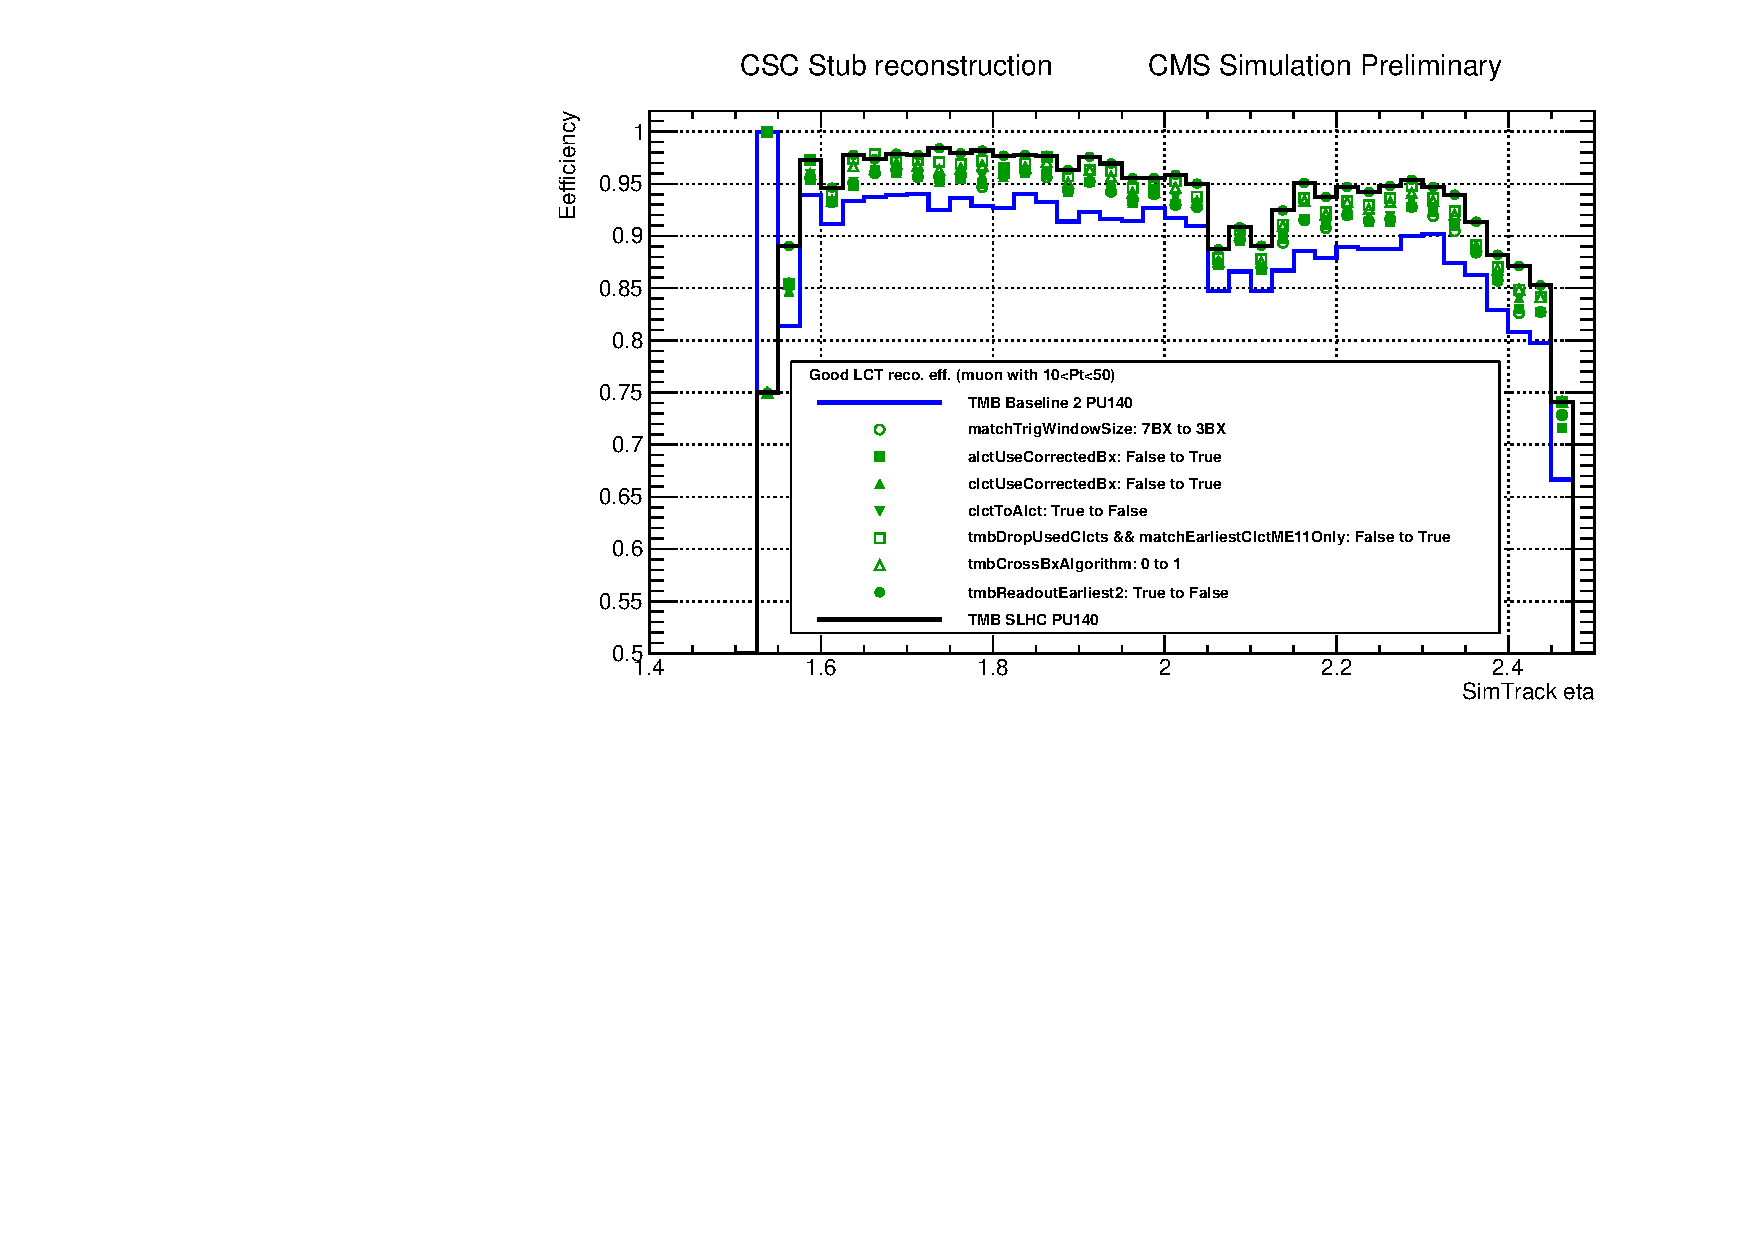
\includegraphics[width=0.98\textwidth]{figures/TMB_improvements_LCT_recoEff.pdf}
\caption{Reconstruction efficiency of a good LCT in ME1 station}
\label{fig:TMB_improvements_LCT_recoEff}
\end{figure}

Improvements on the level of TMB are related to the following configuration parameters (see Sec.~\ref{sec:TMB_conf}):
\begin{itemize}
	\item matchTrigWindowSize: 7BX to 3BX;
	\item tmbReadoutEarliest2: True to False;
	\item alctUseCorrectedBx: False to True
	\item clctUseCorrectedBx: False to True;
	\item clctToAlct: True to False;
	\item tmbDropUsedClcts and matchEarliestClctME11Only: True to False;
	\item tmbCrossBxAlgorithm: 0 to 1.
\end{itemize}

Fig.~\ref{fig:TMB_improvements_LCT_recoEff} shows reconstruction efficiency of a good LCT in ME1 station versus pseudorapidity of the simulated muon for different L1 configurations. The good LCT is defined as LCT consisted of a good ALCT and a good CLCT.

The major improvement in LCT reconstruction efficiency comes from:
\begin{itemize}
	\item changing the size of a window where ALCTs and CLCTs are read out for further correlation betweeb each other;
	\item stopping to read out only the first two CLCTs;
	\item stopping to drop used CLCTs;
	\item stopping to match only to the earliest CLCT.
\end{itemize}

\newpage
